\documentclass[11  pt]{exam} 
\usepackage[lmargin=1in,rmargin=1.75in,bmargin=1in,tmargin=1in]{geometry}  


% For hyperlinking everything
\usepackage{hyperref}
\hypersetup{
	colorlinks=true, %set true if you want colored links
	linktoc=all,     %set to all if you want both sections and subsections linked
	linkcolor=blue,  %choose some color if you want links to stand out
}


\usepackage[latin1]{inputenc}
\usepackage{amsmath}
\usepackage{mathrsfs}  
\usepackage{amsfonts}
\usepackage{amssymb}
\usepackage{graphicx}
\usepackage{subfig}
\usepackage{caption}
\usepackage{algorithm}
%\usepackage{algcompatible}
%\usepackage{algorithmicx}
\usepackage{algpseudocode}

\usepackage{titlesec}
\titleformat{\section}{\fontfamily{lmss}\fontsize{14}{15}\bfseries}{\thesection}{1em}{}
\titleformat{\subsection}{\fontfamily{lmss}\fontsize{12}{15}\bfseries}{\thesubsection}{1em}{}




\usepackage{amsthm}

\newtheoremstyle{noit}
{10pt}% <Space above>
{10pt}% <Space below>
{}% <Body font>
{}% <Indent amount>
{\bfseries}% <Theorem head font>
{.}% <Punctuation after theorem head>
{.5em}% <Space after theorem headi>
{}% <Theorem head spec (can be left empty, meaning `normal')>

\newtheoremstyle{example}
{10pt}% <Space above>
{10pt}% <Space below>
{}% <Body font>
{20pt}% <Indent amount>
{\bfseries}% <Theorem head font>
{.}% <Punctuation after theorem head>
{.5em}% <Space after theorem headi>
{}% <Theorem head spec (can be left empty, meaning `normal')>


\newtheoremstyle{indented}{20pt}{20pt}{\addtolength{\leftskip}{2.5em}}{}{\bfseries}{.}{.5em}{}


\newtheorem{theorem}{Theorem}
\numberwithin{theorem}{section}
\newtheorem{lemma}[theorem]{Lemma}
\newtheorem{corollary}[theorem]{Corollary}
\newtheorem{observation}{Observation}
%\numberwithin{observation}{section}
%\numberwithin{definition}{section}
\newtheorem{conjecture}{Conjecture}
\newtheorem{Qu}{Question}
\newcommand{\QU}{\begin{Qu}\normalfont}

\theoremstyle{noit}
\newtheorem{fact}{Fact}
\newtheorem{definition}{Definition}

\theoremstyle{indented}
\newtheorem{example}{Example}

\theoremstyle{indented}
\newtheorem{problem}{Problem}


%\newenvironment{proof}{\noindent{\bf Proof:} \hspace*{1em}}{
%    \hspace*{\fill} $\Box$ }
%\newenvironment{proof_of}[1]{\noindent {\bf Proof of #1:}
%    \hspace*{1em} }{\hspace*{\fill} $\Box$ }
%\newenvironment{proof_claim}{\begin{quotation} \noindent}{
%    \hspace*{\fill} $\diamond$ \end{quotation}}
\newcommand{\vs}[1]{\vspace{#1}}

\newcommand{\lecture}[2]{
 \noindent
\begin{center}
	\framebox{
		\vbox{
			\hbox to 5.78in { {\bf CSCE 411: Design and Analysis of Algorithms} \hfill  }
			\vspace{2mm}
			\hbox to 5.78in { {\Large \hfill Lecture #1\hfill} }
			\vspace{2mm}
			\hbox to 5.78in { {\it Date: #2 \hfill Lecturer: Nate Veldt} }
		}
	}
\end{center}
\vspace*{4mm}
}


\newcommand{\hw}[2]{
	\noindent
	\begin{center}
		\framebox{
			\vbox{
				\hbox to 5.78in { {\bf CSCE 411: Design and Analysis of Algorithms} \hfill  }
				\vspace{2mm}
				\hbox to 5.78in { {\Large \hfill Homework #1\hfill} }
				\vspace{2mm}
				\hbox to 5.78in { {\it Due date: #2 \hfil} }
			}
		}
	\end{center}
	\vspace*{4mm}
}



\newcommand{\under}[1]{\underline{\hspace{#1}}}
\setlength{\parindent}{0em}

%\usepackage[tagged]{accessibility}

% Graph terms
\newcommand{\vol}{\textbf{vol}}
\newcommand{\cut}{\textbf{cut}}


% Matrices
\newcommand{\mA}{\textbf{A}}
\newcommand{\mB}{\textbf{B}}

% vectors
\newcommand{\ve}{\textbf{e}}
\newcommand{\vx}{\textbf{x}}


% Other
\newcommand{\calN}{\mathcal{N}}

\usepackage{mathtools}
\DeclarePairedDelimiter\ceil{\lceil}{\rceil}
\DeclarePairedDelimiter\floor{\lfloor}{\rfloor}


\newcommand*{\aitem}{ \item[{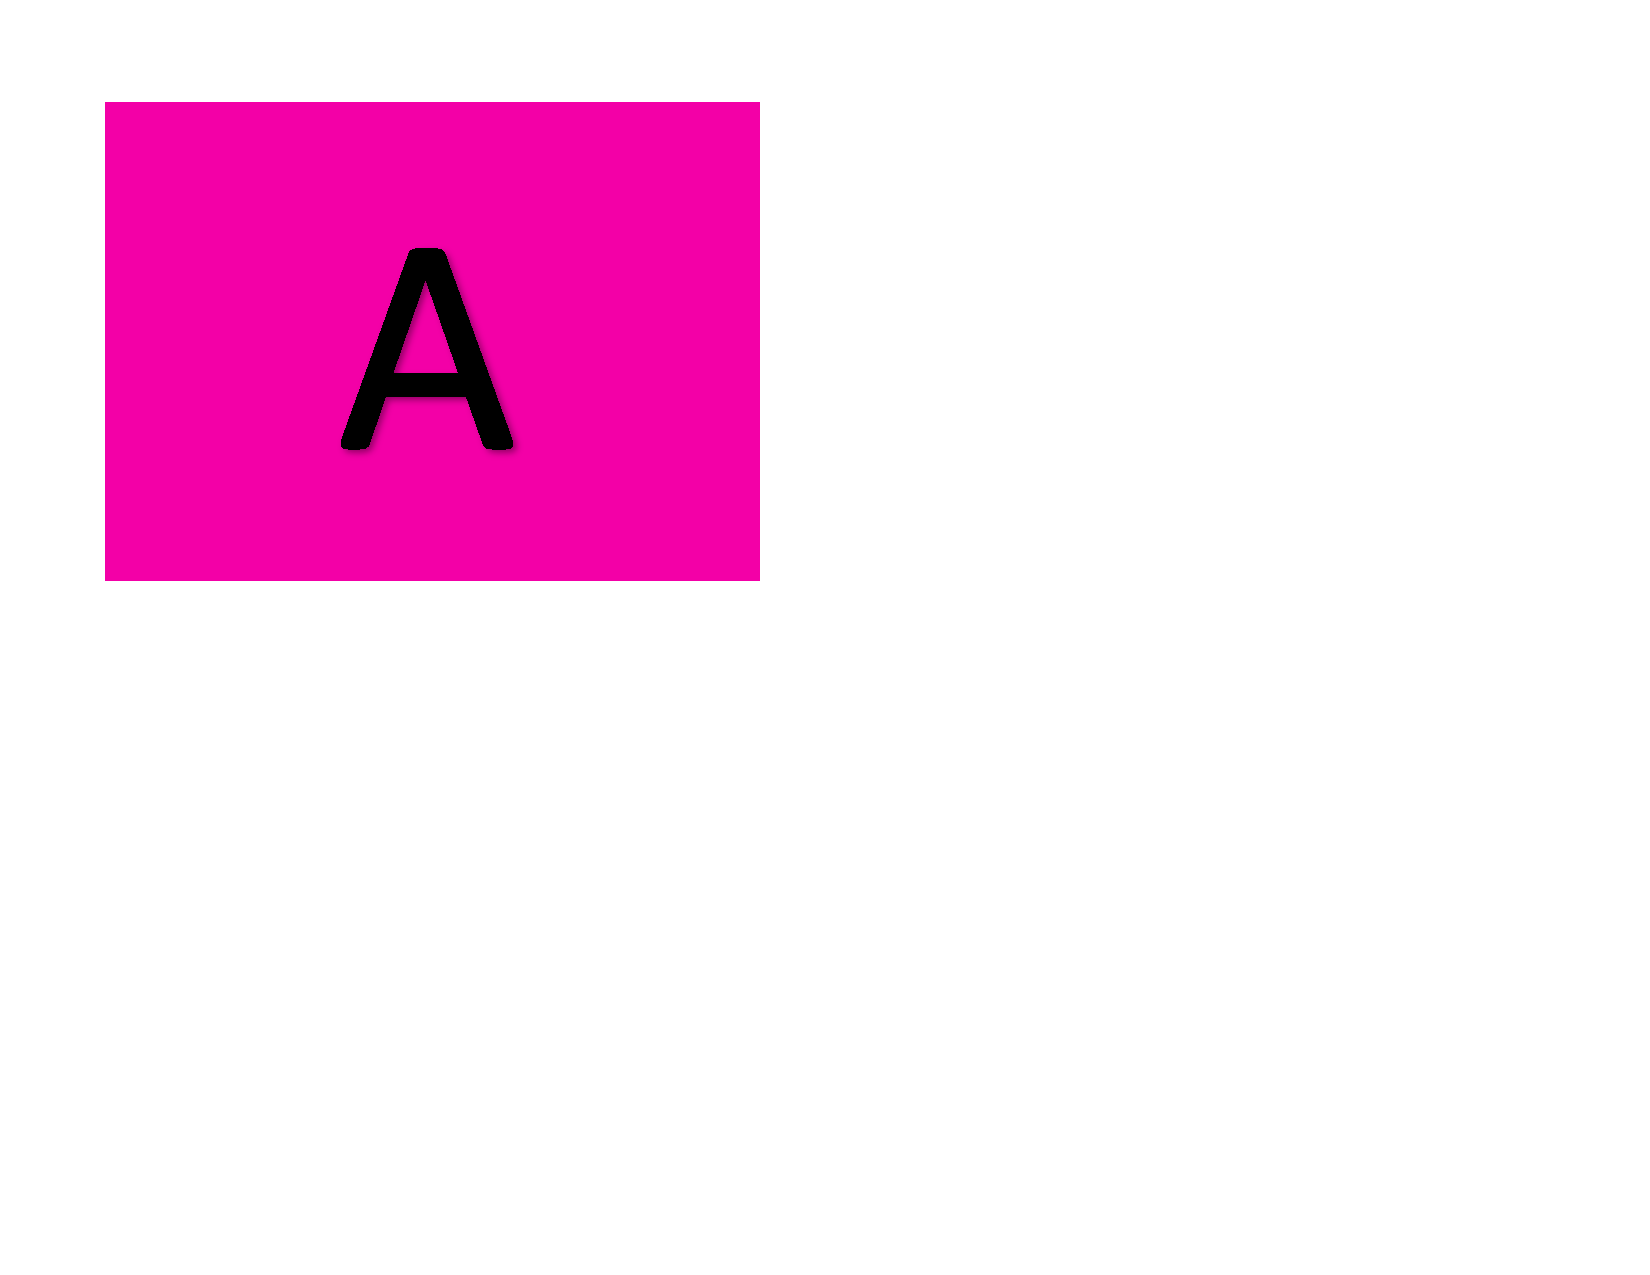
\includegraphics[width=0.8cm,height=0.5cm]{../../Lectures/figures/A}} ]  }
\newcommand*{\bitem}{ \item[{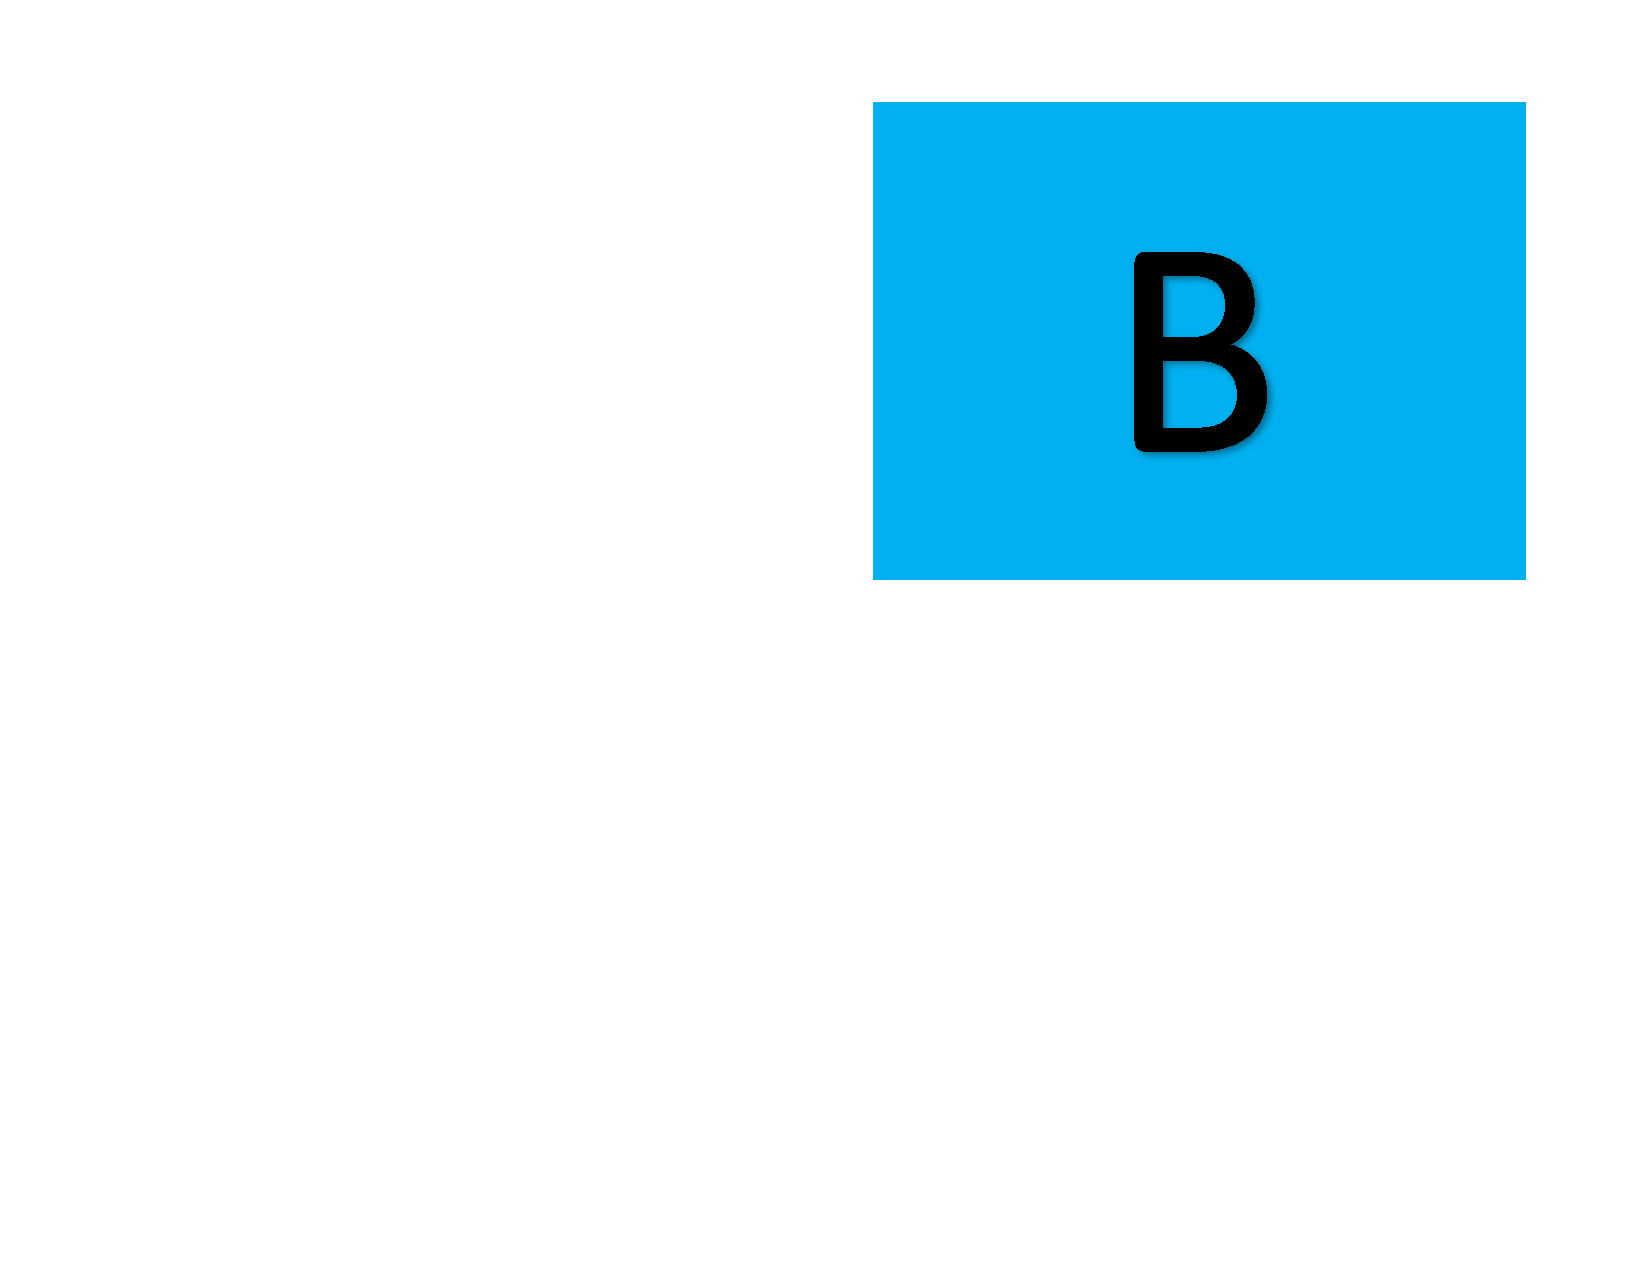
\includegraphics[width=0.8cm,height=0.5cm]{../../Lectures/figures/B}} ]  }
\newcommand*{\citem}{ \item[{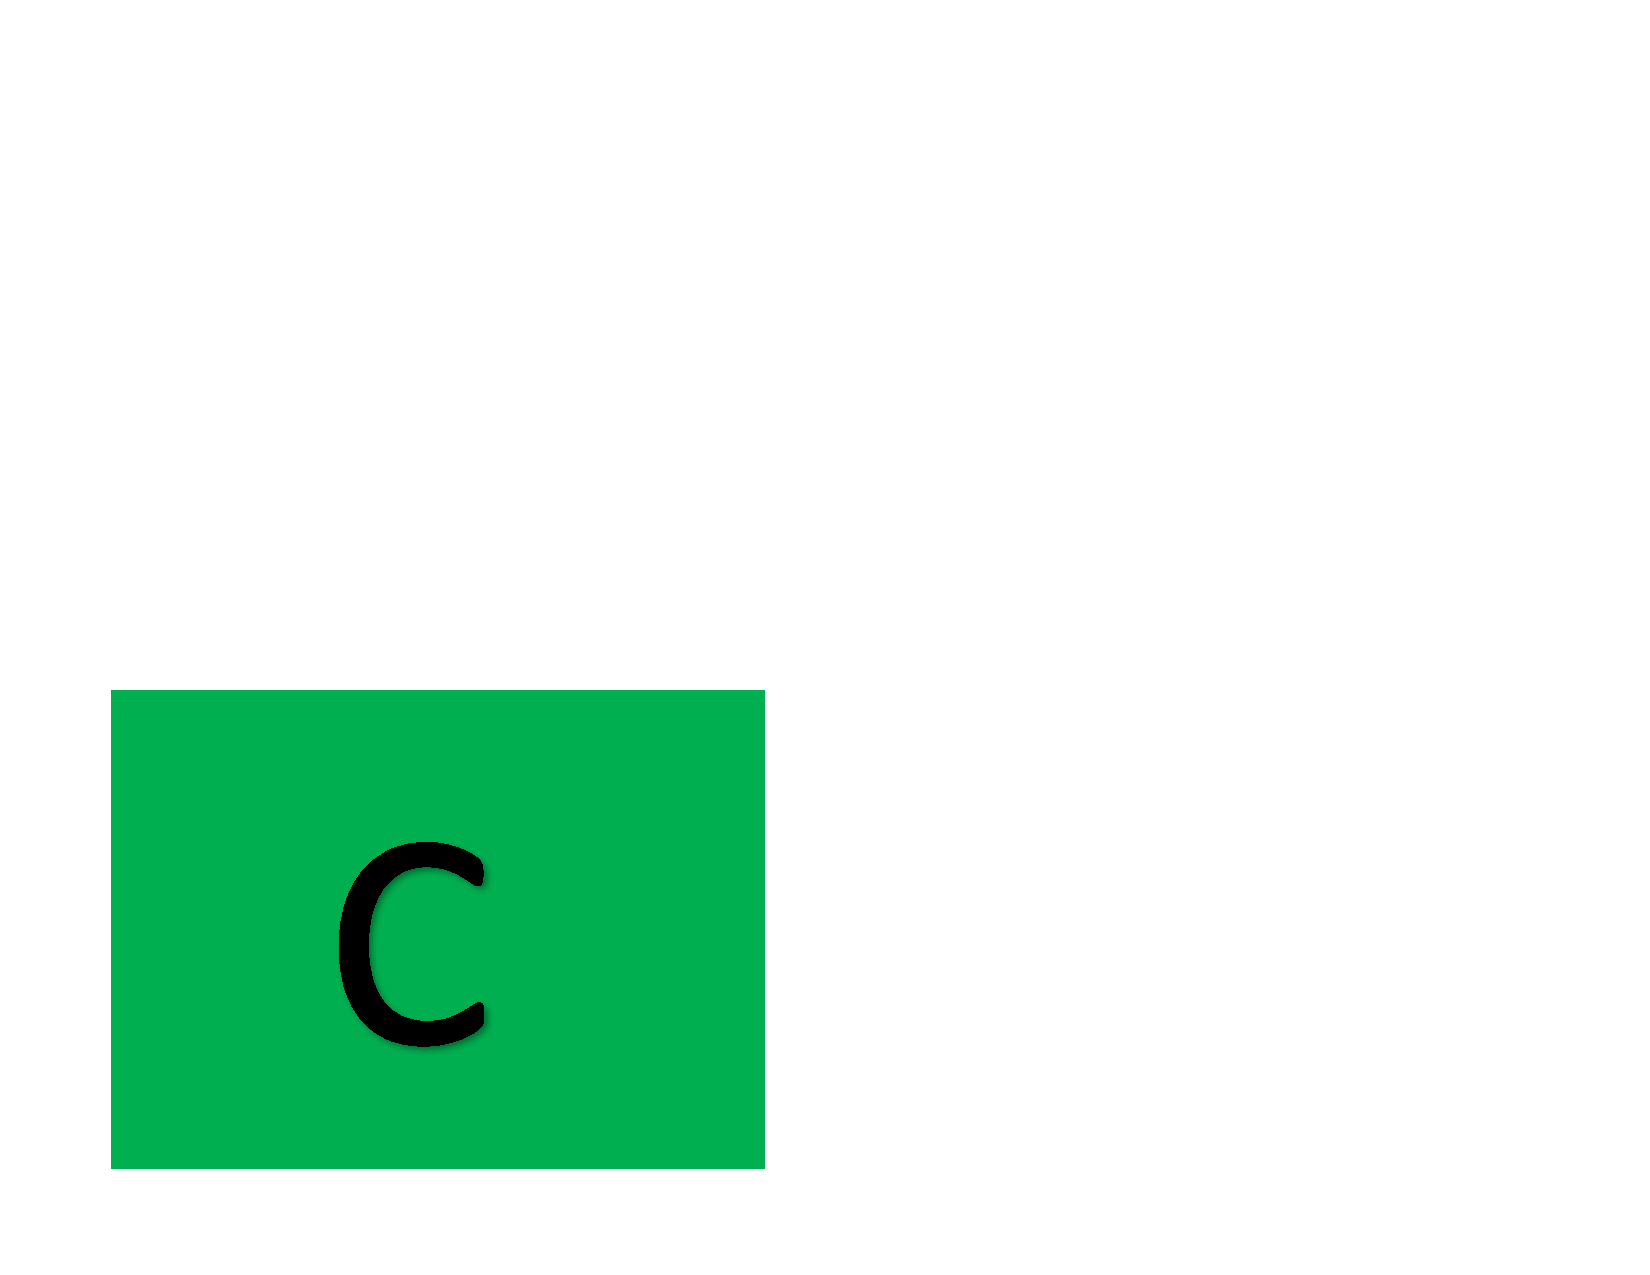
\includegraphics[width=0.8cm,height=0.5cm]{../../Lectures/figures/C}} ]  }
\newcommand*{\ditem}{ \item[{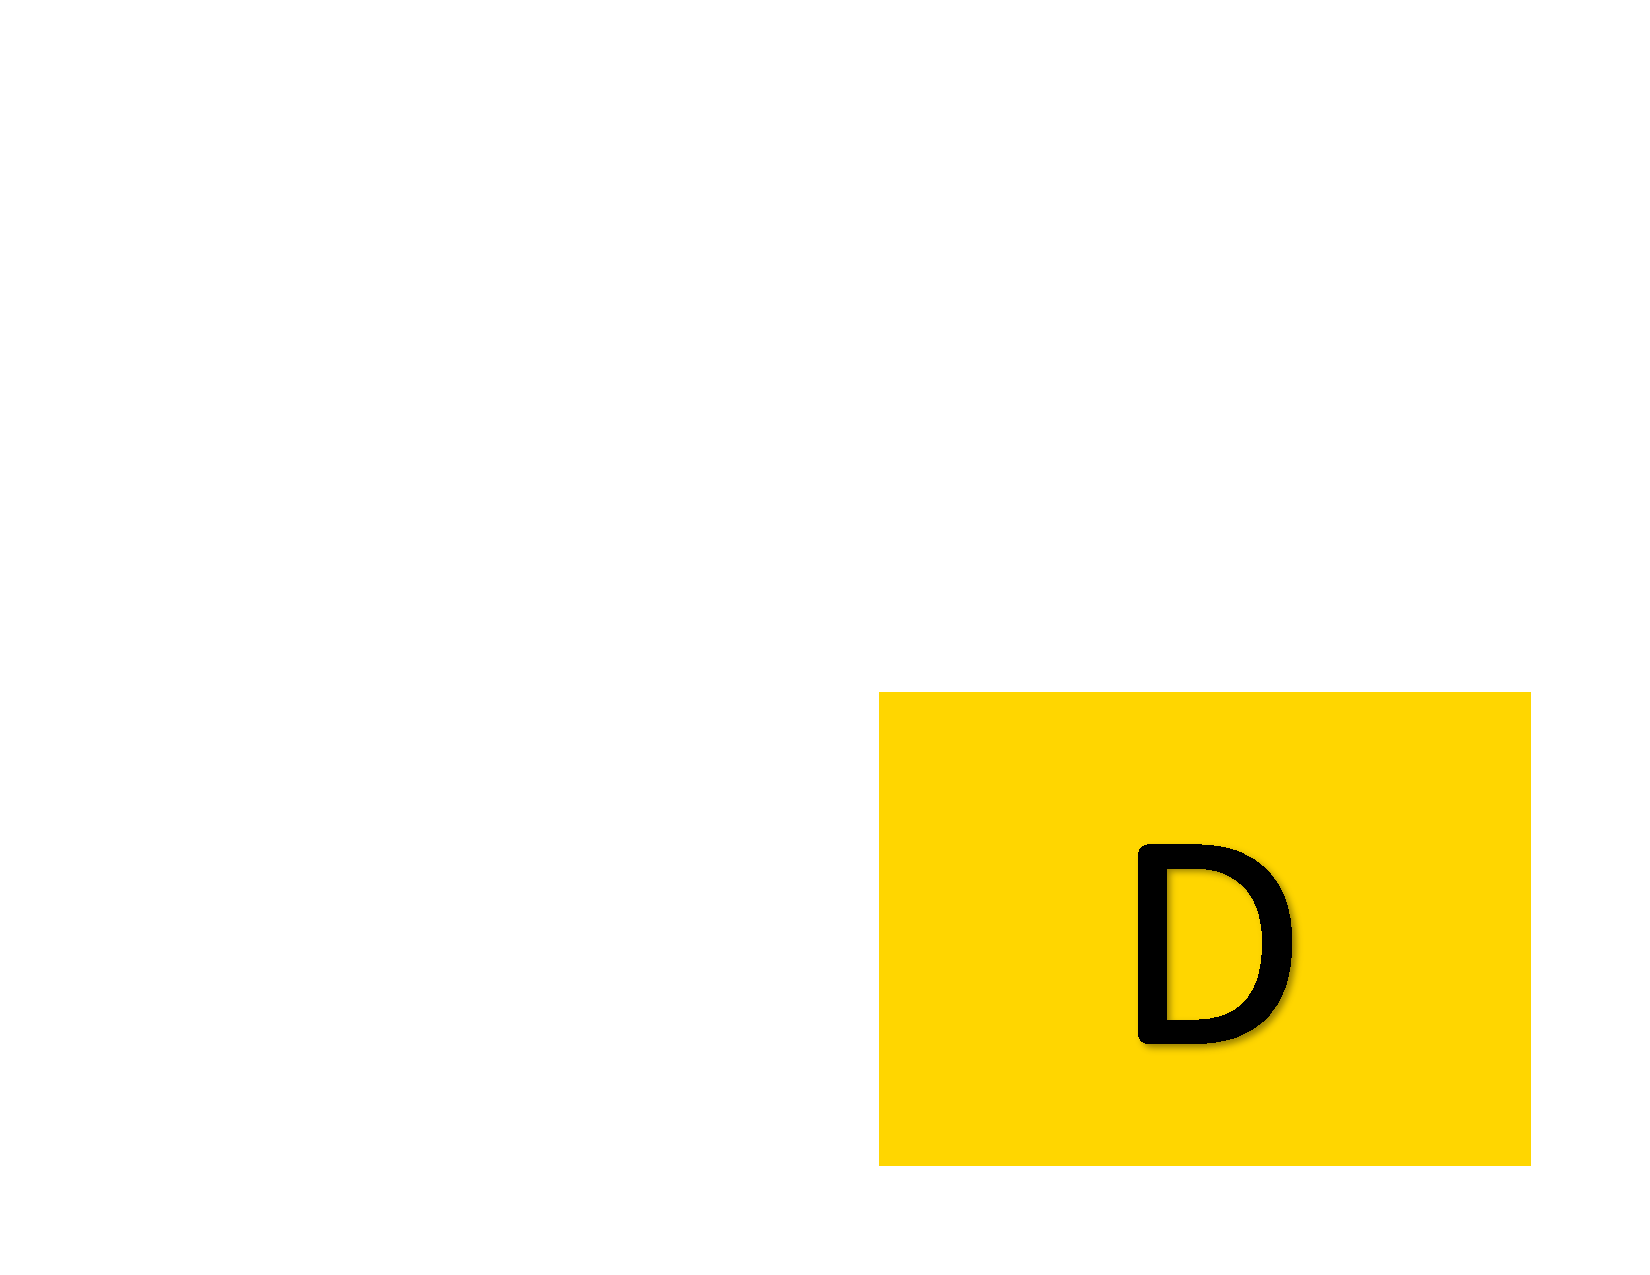
\includegraphics[width=0.8cm,height=0.5cm]{../../Lectures/figures/D}} ]  }
\newcommand*{\eitem}{ \item[{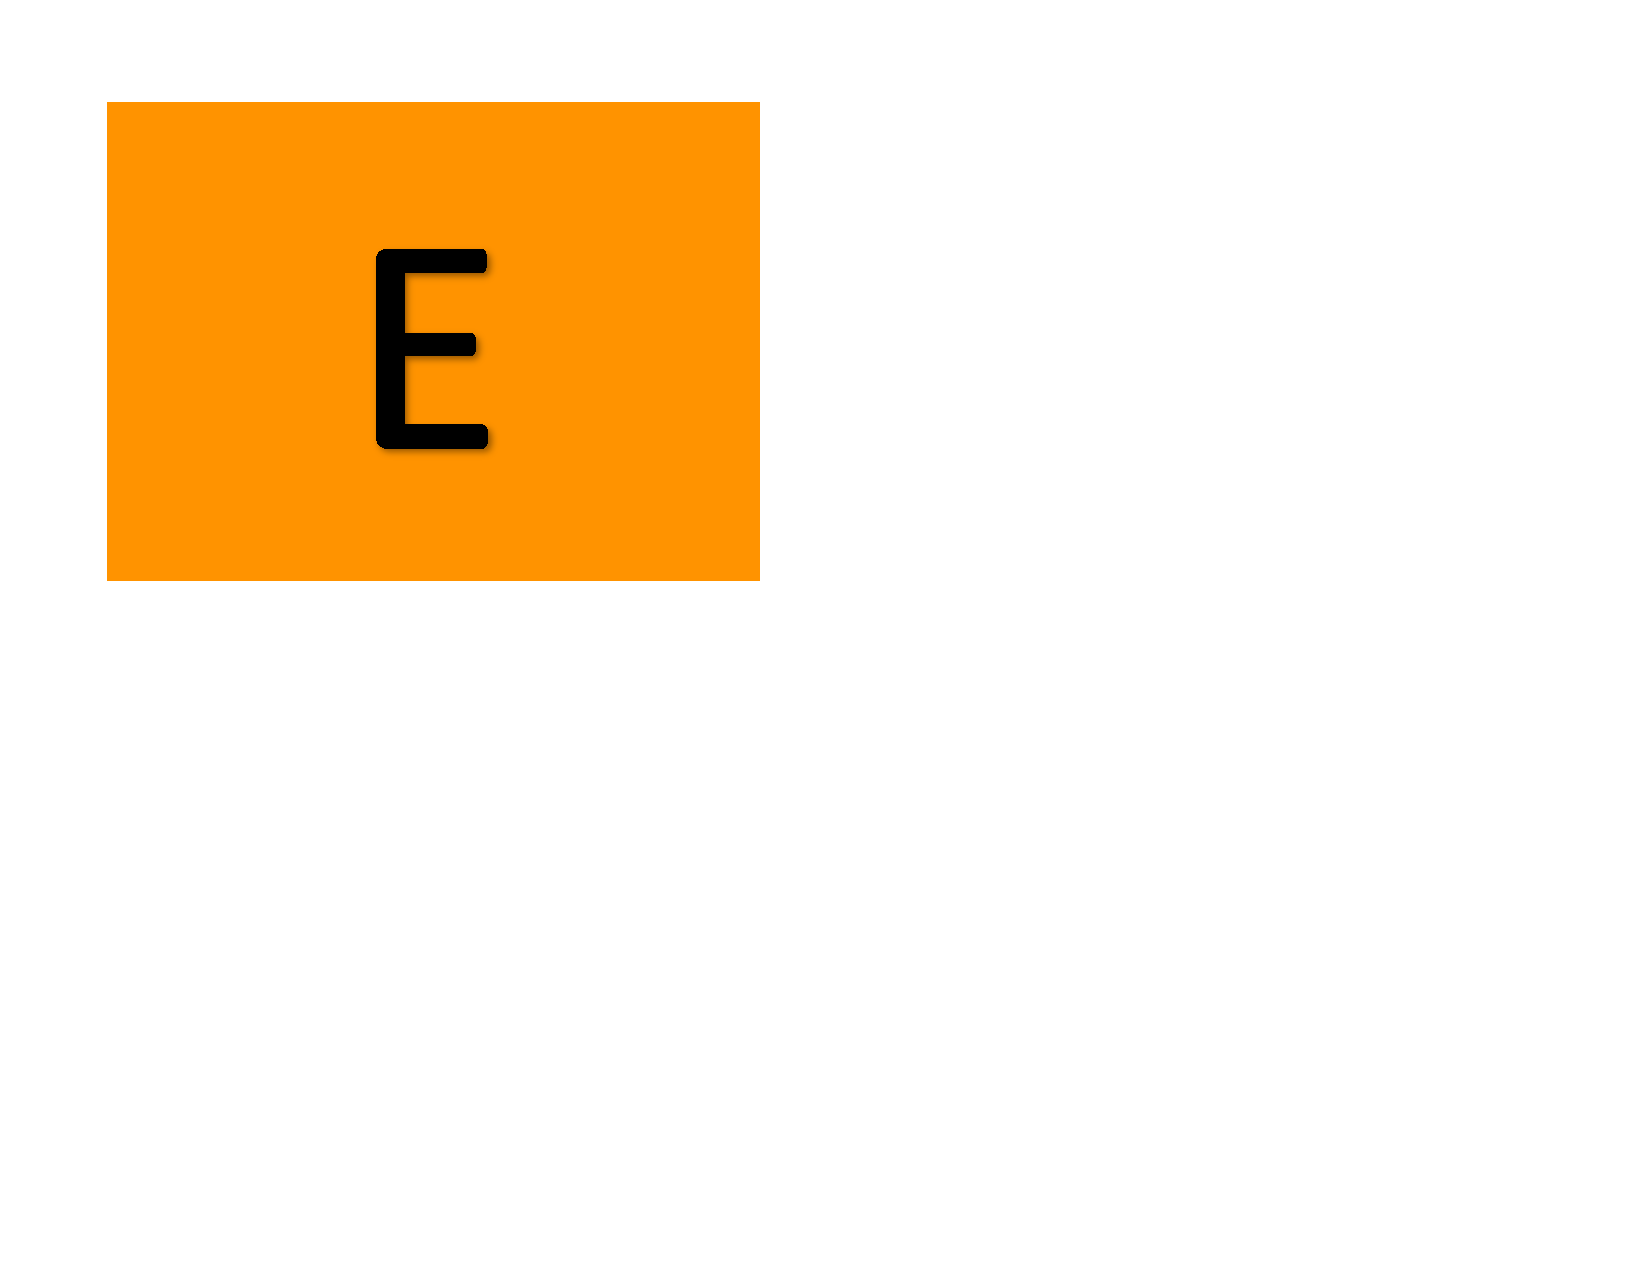
\includegraphics[width=0.8cm,height=0.5cm]{../../Lectures/figures/E}} ]  }
\newcommand*{\fitem}{ \item[{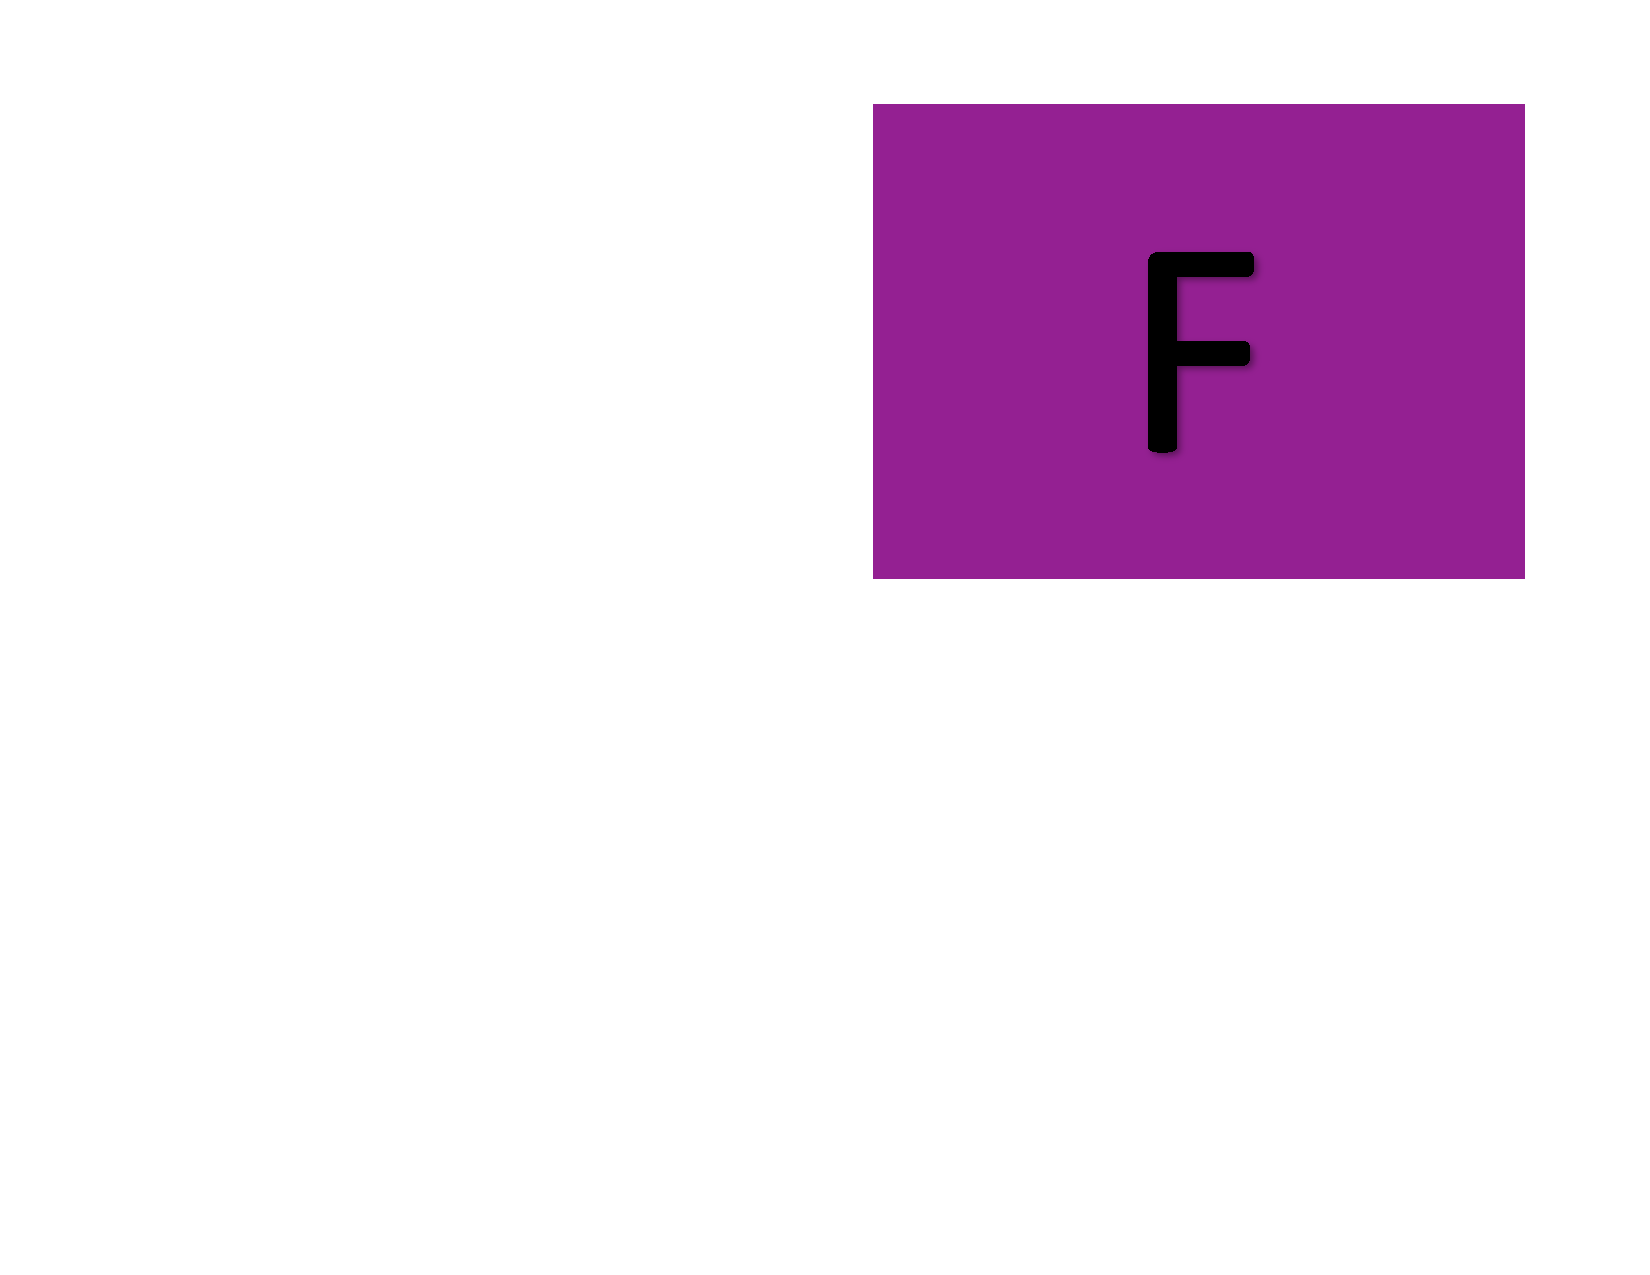
\includegraphics[width=0.8cm,height=0.5cm]{../../Lectures/figures/F}} ]  }


\newcommand{\hide}[1]{\underline{\phantom{#1 #1}}}

\usepackage{setspace}

\onehalfspacing

\begin{document}
	
	
	\lecture{8, Exam 1 Review}{February 11, 2025}
	
	
	\section{Test format and instructions}
	
	\begin{itemize}
		\item 12 multiple choice questions, 3 long answer questions
		\item You do not need to prove something unless you are explicitly asked to prove something
		\item You will be asked to explicitly prove something 
		\item Scratch paper will be provided
		\item No calculators or electronic devices. You will not need them. If you have to do any computations, they will be basic enough to do by hand.
		\item You will put your name on the front page, and put your initials at the top of every other page.
		\item You have been provided with a ``cheat sheet'' with notes that you can use on the test without having to memorize it (including the Master Theorem among other things.) 
	\end{itemize}
	
	\newpage 
	
	\section{Topics Covered on the Exam}
	
	%	These notes go over the main topics we have studied, list questions for you to fill in that you should know about on the test, and give some examples of things you might be required to do on the test.
	%	
	\subsection{Algorithm basics}
	For the whole test, you should be familiar with
	\begin{itemize}
		\item $O$ notation, $\Theta$ notation, $\Omega$ notation, and the differences among them
		\item Basic matrix multiplication
		\item Basic proof strategies (i.e., induction, contradiction)
	\end{itemize}
	
	\subsection{Divide-and Conquer}
	%	Reading: Chapter 4. \\
	
	\textbf{Conceptual questions}
	\begin{itemize}
		\item What properties should hold in order to apply a divide-and-conquer approach?
		\item What are the three steps of a divide-and-conquer method? 
		\item What strategies are there for proving a runtime from a runtime recurrence relation?
		\item What parts of the recurrence relation correspond to the three steps of divide and conquer?
	\end{itemize}
	
	\textbf{Specific problems to know about}
	\begin{itemize}
		\item Merge-sort
		\item Strassen's Algorithm for matrix multiplication
	\end{itemize}
	
	\textbf{Possible types of sample questions} (non-exhaustive!)
	\begin{itemize}
		\item Use different methods to prove runtime guarantees from recurrence relations (e.g., apply the Master Theorem to give a runtime from a recurrence)
		\item Find the recurrence related satisfied by an algorithm
		\item Analyze the runtime of the combine step of a divide-and-conquer method
		\item Provide pseudocode for the combine step of merge sort
	\end{itemize}
	
	\subsection{Dynamic Programming}
	\textbf{Conceptual Questions}
	\begin{itemize}
		\item What properties should hold in order to apply a dynamic programming approach?
		\item How is dynamic programming similar and different from divide-and-conquer?
		\item What are two different approaches for writing code for a dynamic programming algorithm?
	\end{itemize}
	
	\textbf{Specific problems to know about}
	\begin{itemize}
		\item Fibonacci
		\item Rod-cutting
		\item Matrix Chain Multiplication
		\item Min cost path in a grid
	\end{itemize}
	
	\textbf{Possible types of sample questions} (non-exhaustive!)
	\begin{itemize}
				\item Answer some variant of the conceptual questions asked above
				\item Analyze a variation or application of one of the three problems we considered
		\item Provide pseudocode for a dynamic programming version of an algorithm (could be either version of dynamic programming)
		\item Identify when dynamic programming is right for a problem
		\item Give a recurrence relationship for a dynamic programming algorithm
		\item Analyze a runtime based on a recurrence relationship
		\item Prove/explain why overlapping subproblems holds for a certain problem
	\end{itemize}
	
	\subsection{Greedy Algorithms}
	\textbf{Conceptual Questions}
	\begin{itemize}
		\item What properties should hold in order to apply a greedy algorithm?
		\item How is this similar to and different from other algorithmic paradigms?
		\item What is an overall strategy for applying greedy approach to a problem?
	\end{itemize}
	
	\textbf{Problems to know about}
	\begin{itemize}
		\item Activity subset selection problem
		\item The coin change problem
		\item Optimal prefix code problem
		\item Fractional knapsack problem
	\end{itemize}
	
	\textbf{Possible types of sample questions} (non-exhaustive!)
	\begin{itemize}
		%		\item Answer some variant of the conceptual questions asked above
		%		\item Analyze a variation or application of one of the three problems listed above
		\item Provide or analyze pseudocode for a greedy algorithm, e.g., coin change, activity subset selection
		\item Prove that a greedy strategy is optimal for a certain type of problem
		\item Prove that a greedy strategy is \emph{not} optimal
		\item Identify when a greedy algorithm is right for a problem
	\end{itemize}
	
	\subsection{Amortized Analysis}
	\textbf{Conceptual Questions}
	\begin{itemize}
		\item What is the definition of amortized analysis?
		\item How does it differ from other runtime analyses?
		\item What three strategies did we cover for amortized analysis, and how does each one work? What do you have to choose/set/show for each one?
		\item How are different strategies different?
	\end{itemize}
	
	\textbf{Problems to know about}
	\begin{itemize}
		\item Multipop stack
		\item Binary counter increment problem
	\end{itemize}
	
	\textbf{Possible types of sample questions} (non-exhaustive!)
	\begin{itemize}
		%		\item Answer some variant of the conceptual questions asked above
		%		\item Analyze a variation or application of one of the three problems listed above
		\item Prove that a certain choice of amortized costs is bounded above
		\item Prove that a certain choice of amortized costs bounds the actual cost
		\item Identify the right potential function using the potential method
		\item Perform an aggregate analysis of an algorithm
	\end{itemize}
	
	
	\section{Tips on How to do a Runtime Analysis}
	
	\begin{itemize}
		\item \textbf{Simple Iterative Algorithms}
		\begin{itemize} 
			\item Bound number of iterations
			\item Bound runtime for each iteration, multiply by number of iterations
		\end{itemize}
		\item \textbf{Divide and conquer}
		\begin{itemize} 
			\item Obtain a recurrence relationship
			\item Confirm that subproblems do not overlap
			\item Apply Master Theorem, or another approach
		\end{itemize}
		\item \textbf{Dynamic programming}
		\begin{itemize} 
			\item Prove recurrence relationship between subproblems
			\item Confirm problems overlap
			\item Design an implementation that only solves each subproblem once. Given that each problem is only solved once, what is the overall runtime cost?
		\end{itemize}
		\item \textbf{Amortized Analysis, for iterative method}
		\begin{itemize} 
			\item Aggregate analysis: bound total cost, divide by number of iterations (rather than multiplying number of iterations by maximum iteration cost)
			\item There are two other methods...see practice problems and lecture notes for overview.
		\end{itemize}
	\end{itemize}
	\newpage
	
	\section{Practice Problems}
	
	\begin{questions}
		
		\question What are the three steps of a divide-and-conquer method? Given examples.
		
		\question Describe what steps are needed to prove an amortized runtime analysis using the potential method and the accounting method.
		
		\question What two properties should be satisfied by a problem in order to use a greedy method?
		
		\question What is the strategy we have seen for proving that a greedy method is optimal?
		
		\question Consider the following recurrence:
		\begin{equation*}
			c[i,j] =\begin{cases}
				0 & \text{ if $i = 0$ or $j = 0$} \\
				c[i-1, j-1] + 1 & \text{ if $i,j > 0$ and \textsc{Special Condition} holds}\\
				\max \{ c[i,j-1], c[i-1,j]\} & \text{ if $i,j > 0$ and \textsc{Special Condition} does not hold}.
			\end{cases}
		\end{equation*}
		where $c[i,j]$ is a subproblem of a problem that can be solved via dynamic programming, and is defined for every $i$ and $j$ such that $1 \leq i \leq g$ and $1 \leq j \leq p$. What is the runtime for computing $c[g,p]$ if it takes $O(1)$ time to check \textsc{Special Condition}?
		
		\question Consider the following recurrence relations
		\begin{align*}
			T(n) &= 4T(n/4) + n \\
			T(n) &= 7T(n/2) + n^2 \\
			T(n) &= 3T(n/2) + n^5 \log n\\
			T (n) &= 3T (n/3) + n \log n 
		\end{align*}
		What runtime for this method does the Master Theorem give in each case? Make sure you are aware of situations where the Master Theorem does not apply. You can find other versions of the Master Theorem from other sources, but we will restrict to using the version in our textbook (as presented in class).
		
		\textbf{Reviewing other homework problems is the next best way to prepare!}
		
	\end{questions}
\end{document}
